\scanpage{22}
\diagram{\begin{array}{rll}
\texttt{1}&\texttt{//PREDONTA JOB CNU0049-PREDONT,TIME=(0,3),CLASS=R}&\texttt{JOB 1085}\\
\texttt{2}&\texttt{// EXEC ASMFCL}&\texttt{00000020}\\
\texttt{3}&\texttt{XXASMFCL PROC MAC='SYS1.MACLIB',MAC1='CNU1.MACLIB'}&\texttt{00010071}\\
\texttt{}&\texttt{*** REFER SYS1.PROCLIB(ASMFCL)}&\texttt{00020000}\\
\texttt{}&\texttt{*** COMPID SYSTEM}&\texttt{00030000}\\
\texttt{}&\texttt{*** DOC THIS PROCEDURE EXECUTES THE ASSEMBLER AND THE LINKAGE}&\texttt{00040000}\\
\texttt{}&\texttt{*** EDITOR.}&\texttt{00050000}\\
\texttt{}&\texttt{***}&\texttt{00060000}\\
\texttt{4}&\texttt{XXASM EXEC PGM=IFOX00,PARM=OBJ}&\texttt{00070075}\\
\texttt{5}&\texttt{//ASM.SYSLIB DD DSN=CNU2.MODULEF.UTIMS,DISP=SHR}&\texttt{00000030}\\
\texttt{}&\texttt{X/SYSLIB DD DSN=\&MAC,DISP=SHR}&\texttt{00080070}\\
\texttt{6}&\texttt{// DD DSN=SYS1.MACLIB,DISP=SHR       -}&\texttt{00000040}\\
\texttt{}&\texttt{X/ DD DSN=\&MAC1,DISP=SHR}&\texttt{00090070}\\
\texttt{7}&\texttt{// DD DSN=CNU1.MACLIB,DISP=SHR}&\texttt{00000050}\\
\texttt{8}&\texttt{XXSYSUT1 DD DSN=\&\&SYSUT1,UNIT=VIO,SPACE=(CYL,(20,20))}&\texttt{00091076}\\
\texttt{9}&\texttt{XXSYSUT2 DD DSN=\&\&SYSUT2,UNIT=VIO,SPACE=(CYL,(10,10))}&\texttt{00092076}\\
\texttt{10}&\texttt{XXSYSUT3 DD DSN=\&\&SYSUT3,UNIT=VIO,SPACE=(CYL,(5,5))}&\texttt{00093076}\\
\texttt{11}&\texttt{XXSYSPRINT DD SYSOUT=*,DCB=BLKSIZE=1089}&\texttt{00130072}\\
\texttt{12}&\texttt{XXSYSPUNCH DD DUMMY}&\texttt{00140071}\\
\texttt{13}&\texttt{XXSYSGO DD DSN=\&\&OBJSET,UNIT=SYSDA,SPACE=(80,(200,50)),}&\texttt{00150070}\\
\texttt{}&\texttt{XX DISP=(MOD,PASS)}&\texttt{00160000}\\
\texttt{14}&\texttt{//ASM.SYSIN DD DSN=CNU2.MODULEF.UTIAS(IAND),DISP=SHR}&\texttt{00000060}\\
\texttt{15}&\texttt{XXLKED EXEC PGM=IEWL,PARM=(XREF,LET,LIST,NCAL),REGION=128K,}&\texttt{00170070}\\
\texttt{}&\texttt{XX COND=(8,LE,ASM)}&\texttt{00180071}\\
\texttt{16}&\texttt{XXSYSLIN DD DSN=\&\&OBJSET,DISP=(OLD,DELETE)}&\texttt{00190070}\\
\texttt{17}&\texttt{XX DD DDNAME=SYSIN}&\texttt{00200070}\\
\texttt{18}&\texttt{//LKED.SYSLMOD DD DSN=CNU2.MODULEF.UTIA(IAND),DISP=SHR}&\texttt{00000070}\\
\texttt{}&\texttt{X/SYSLMOD DD DSN=\&\&GOSET(GO),UNIT=3350,SPACE=(1024,(50,20,1)),}&\texttt{00210073}\\
\texttt{}&\texttt{XX DISP=(MOD,PASS)}&\texttt{00220000}\\
\texttt{19}&\texttt{XXSYSUT1 DD DSN=\&\&SYSUT1,UNIT=VIO,SPACE=(1024,(50,20))}&\texttt{00230070}\\
\texttt{20}&\texttt{XXSYSPRINT DD SYSOUT=*,DCB=(RECFM=FB,LRECL=121,BLKSIZE=1210)}&\texttt{00240072}\\
\texttt{}&\texttt{//}&\texttt{00000080}
\end{array}}

\diagram{\begin{tikzcd}
A \arrow[r,"\unsure{a}"] \arrow[d,very thick,"\mathrm{cof}"'] & X \arrow[d,very thick,"p"]\\
A\times I \arrow[r,"h"'] \arrow[ur,very thick] & Y
\end{tikzcd}}
\figure{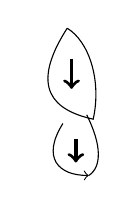
\begin{tikzpicture}[scale=.55]
\draw (0,2.8) .. controls (-.9,1.4) and (-.3,.9) .. (.6,.7) .. controls (.8,1.6) and (.5,2.5) .. (0,2.8);
\draw[->,very thick] (.1,2.1)--(.1,1.4);
\draw[->] (-.1,.6) .. controls (-.6,-.2) and (-.2,-.6) .. (.5,-.6);
\draw (.45,.8) .. controls (.8,.1) and (.8,-.4) .. (.5,-.6);
\draw[->,very thick] (.2,.25)--(.2,-.3);
\end{tikzpicture}}
\margin{$\unsure{\mathrm{fib}}$}
\diagram{\begin{tikzcd}
A & X \arrow[l]\\
A^I \arrow[u,"\deleted{\unsure{\partial_1}}\partial_0"'] & Y \arrow[l,very thick] \arrow[u,very thick,"\mathrm{cofib.}"]
\end{tikzcd}}
\figure{\begin{tikzpicture}
\draw (0,0)--(.3,.8)--(.4,.4);
\node at (2,0) {$\unsure{Y_x}$};
\end{tikzpicture}}
\diagram{\begin{tikzcd}
A \arrow[r,very thick] \arrow[d,very thick] & X \arrow[d,very thick]\\
B \arrow[r] \arrow[ur,very thick] & Y
\end{tikzcd}}
\mspage{21}
